\chapter{Estructurales}
\section{Introducción}
contenido...
%-----------------------------------------------------------------
\newpage
\section{Adaptador}
contenido...
\subsection{Caso de Uso Realización del Modelo}
contenido...
\begin{figure}[th!]
	\centering
	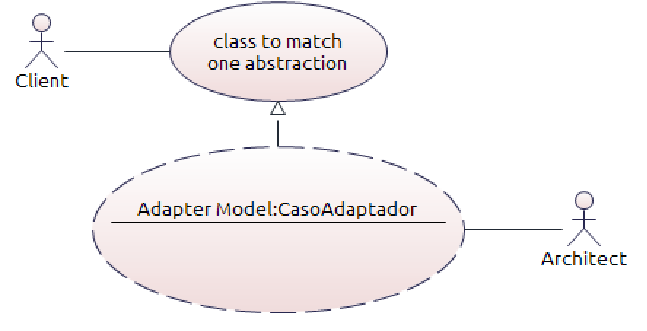
\includegraphics[width=0.7\linewidth]{arquitectura_diseno/imgs/MCU_Adaptador}
	\caption{diagrama de caso de uso}
\end{figure}
\newpage
\subsection{Secuencia Extendida del Modelo}
contenido...
\begin{figure}[th!]
	\centering
	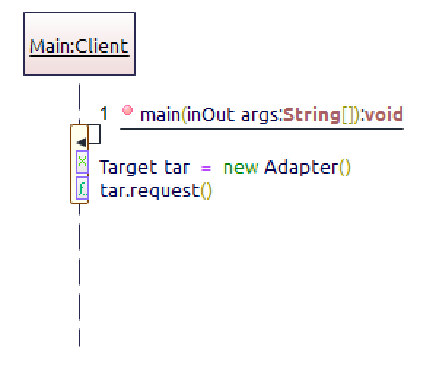
\includegraphics[width=0.7\linewidth]{arquitectura_diseno/imgs/MSE_Adaptador}
	\caption{diagrama de secuencia}
\end{figure}
\newpage
\subsection{Clases  del Modelo}
contenido...
\begin{figure}[th!]
	\centering
	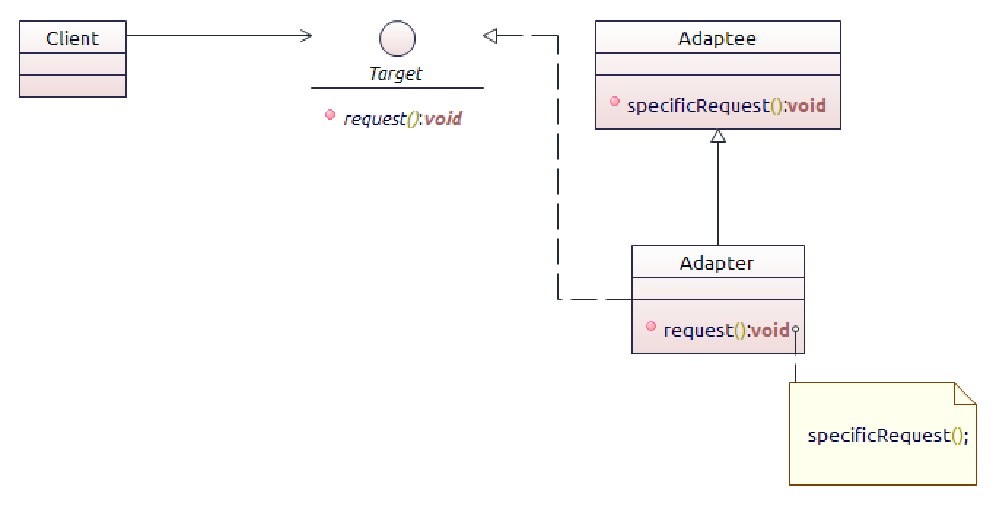
\includegraphics[width=0.7\linewidth]{arquitectura_diseno/imgs/MCL_Adaptador}
	\caption{diagrama de clases}
\end{figure}
\newpage
\subsection{Código Fuente}
%\lstinputlisting[]{C:/a/Client.java}
%\lstinputlisting[]{C:/a/Target.java}
%\lstinputlisting[]{C:/a/Adaptee.java}
%\lstinputlisting[]{C:/a/Adapter.java}
%-----------------------------------------------------------------
\newpage
\subsection{Caso de Uso Realización del Caso}
contenido...
\begin{figure}[th!]
	\centering
	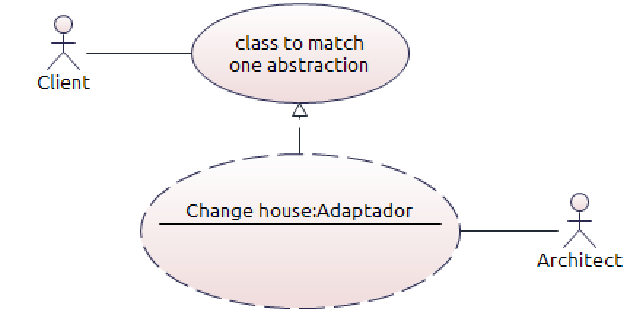
\includegraphics[width=0.7\linewidth]{arquitectura_diseno/imgs/CCU_Adaptador}
	\caption{diagrama de caso de uso}
\end{figure}
\newpage
\subsection{Secuencia Extendida del Caso}
contenido...
\begin{figure}[th!]
	\centering
	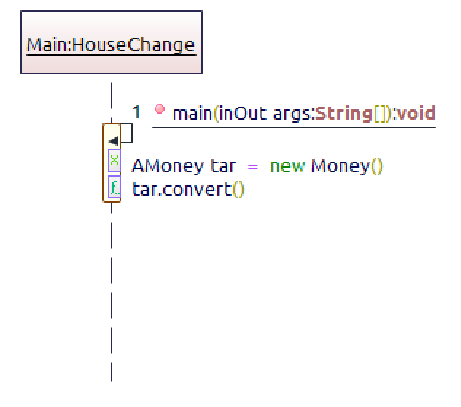
\includegraphics[width=0.7\linewidth]{arquitectura_diseno/imgs/CSE_Adaptador}
	\caption{diagrama de secuencia}
\end{figure}
\newpage
\subsection{Clases  del Caso}
contenido...
\begin{figure}[th!]
	\centering
	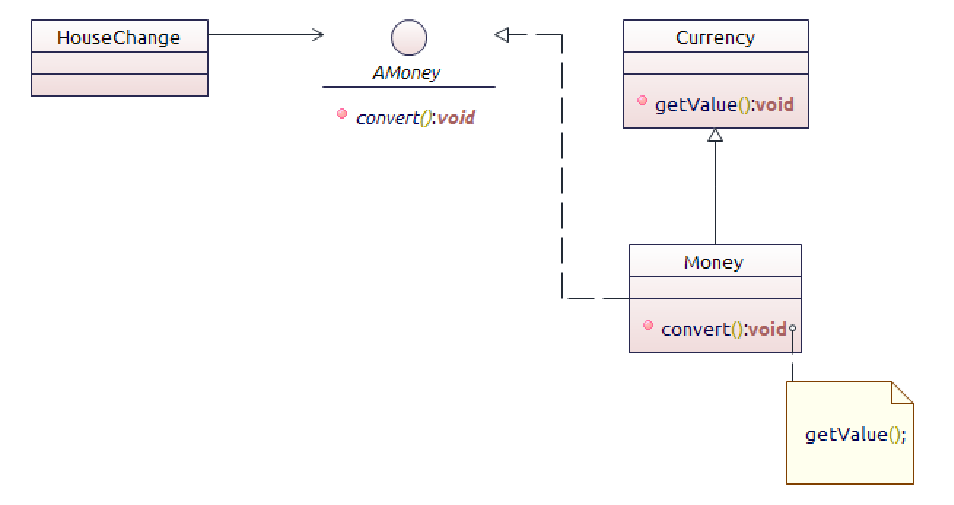
\includegraphics[width=0.7\linewidth]{arquitectura_diseno/imgs/CCL_Adaptador}
	\caption{diagrama de clases}
\end{figure}
\newpage
\subsection{Código Fuente}
%\lstinputlisting[]{C:/a/HouseChange.java}
%\lstinputlisting[]{C:/a/AMoney.java}
%\lstinputlisting[]{C:/a/Currency.java}
%\lstinputlisting[]{C:/a/Money.java}
